\textbf{Agenda}

Pada chapter ini kita akan membahas beberapa topik tentang 
Casting dan Database, adapun topik yang akan dibahas
adalah

\minitoc

\section{Mengenal Casting}\label{mengenal-casting}

Casting merupakan mekanisme dimana programmer dapat secara permanen atau
temporary mengubah interpretasi compiler terhadap suatu obyek. Perubahan
ini tidak benar-benar terjadi, namun hanya cara pandang compiler saja
yang diubah. Casting diimplementasikan dalam bentuk ``casting
operator''. Mengapa butuh casting? Dalam dunia pemrograman yang semuanya
jelas (strong type language) dan jika kita hanya menggunakan satu bahasa
pemrograman saja, seperti C++, maka kita tidak membutuhkan operator
casting. Namun kenyataannya pada dunia nyata yang kita hadapi, banyak
bahasa pemrograman, banyak vendor-vendor berbeda-beda sehingga kode /
modul yg dihasilkan jg berbeda-beda. Hal ini menyebabkan
compiler-compiler bahasa pemrograman tertentu, termasuk C++ juga harus
diubah interpretasinya dengan cara lain sehingga mampu melakukan
kompilasi dan menghasilkan hasil yang kompatibel.

Contoh nyatanya terdapat pada bahasa C dan C++. Pada bahasa C tidak
terdapat tipe data bool (boolean) sehingga kita harus menggunakan kata
kunci typedef.

\begin{lstlisting}[language=c++, numbers=none]
typedef unsigned int BOOL;
BOOL mybool = 0;
BOOL isTrue(){
return mybool;
}
\end{lstlisting}

Pada contoh diatas maka kita harus membuat tipe data baru bertipe
unsigned int yang kita definisikan sebagai BOOL. Nah setelah kita
mendefinisikan tipe data baru BOOL pada C, bagaimana jika kemudian
dikembangkan dengan bahasa C++? Kita harus melakukan konversi BOOL pada
bahasa C ke bahasa C++, dimana bahasa C++ sudah ada tipe data bool yang
tentunya berbeda ``persepsi'' dengan BOOL dari bahasa C. Maka dari itu
dilakukan casting. Berikut adalah contoh castingnya:

\begin{lstlisting}[language=c++, numbers=none]
bool hasilku = (bool) isTrue(); // C-Style cast
\end{lstlisting}

\section{Data Type Casting (Conversion)}\label{data-type-casting-conversion}

Mengubah sebuah ekspresi dari tipe yang diberikan dalam jenis lain
dikenal sebagai tipe-casting. Konversi tersebut ada dua jenis:

\subsection{Implicit conversion}\label{implicit-conversion}

Jenis ini tidak membutuhkan operator khusus. Tipe data yang jangkauannya
besar biasanya dapat dikonversi ke tipe data yang jarak jangkauannya
lebih kecil secara otomatis dengan cara pemotongan nilai otomatis.
Kemudian variabel yang tipe datanya berjarak jangkauan besar juga dapat
menerima data dari variabel yang bertipe data berjarak jangkauan kecil.

\textbf{Contoh:}

\begin{lstlisting}[language=c++, numbers=none]
short a=2000;
int b;
b=a;
\end{lstlisting}

Pada contoh diatas, tipe data \texttt{short} yang berjarak jangkau kecil
dapat ditampung oleh tipe data \texttt{int} yang jarak jangkaunya lebih
besar, walaupun tipe datanya berbeda. Hal ini karena keduanya sama-sama
data numerik dan memang termasuk dalam konversi implisit. \emph{Implisit
conversion} juga dapat diterpakan pada \emph{constrctor} sebuah
\emph{class}, sehingga ketika kita memanggil konstruktor tersebut, maka
konversi akan dilakukan. Contoh:

\begin{lstlisting}[language=c++, numbers=none]
class A {
};
class B {
public:
B (A a)
{
}
};
\end{lstlisting}

Proses instansiasi adalah:

\begin{lstlisting}[language=c++, numbers=none]
A a;
B b=a;
\end{lstlisting}

Pada contoh diatas, terlihat bahwa ketika kita membuat obyek class B,
maka otomatis konstruktor class B dijalankan dan menerima parameter
obyek A. Sehingga kita bisa memasukkan parameter bertipe class A kedalam
class B.

\subsection{Explicit conversion}\label{explicit-conversion}

Konversi tipe ini harus dituliskan pada kode program dengan menggunakan
tanda kurung.

\textbf{Sintaks:}

\begin{lstlisting}[language=c++, numbers=none]
(<type>)<value>
\end{lstlisting}

\textbf{Contoh:}

\begin{lstlisting}[language=c++, numbers=none]
short a=2000;
int b;
b = (int) a; // c-like cast notation
b = int (a); // functional notation
\end{lstlisting}

Cara pertama dengan menegunakan \emph{C-cast like notation}. Pada contoh
diatas, kita memaksa / mengcasting variabel a yang bertipe
\texttt{short} agar diperlakukan seperti tipe data \texttt{integer}
dengan cara memberi tanda kurung (int) sebelum variabel a. Dengan
demikian variabel a akan dianggap / diperlakukan oleh kompiler menjadi
tipe data integer dan bisa di assign ke dalam variabel b yang bertipe
integer.

Cara kedua adalah menggunakan \emph{functional notation} dimana kita
bisa memaksa variabel a yang bertipe \texttt{short} diperlakukan menjadi
\texttt{integer} dengan cara menuliskan kata \texttt{int} kemudian
diberi tanda kurung pada variabel a sehingga variabel a bisa di assign
ke dalam variabel b yang bertipe integer.

\subsubsection*{Contoh Explicit Casting pada Tipe Data Numerik.}

Tulislah kode berikut:

\begin{lstlisting}[language=c++, caption=Explicit Casting pada Tipe Data Numerik]
#include <QtCore/QCoreApplication>
#include <iostream>
using namespace std;
int main(int argc, char *argv[])
{
QCoreApplication a(argc, argv);
int aa=5;
int bb=2;
float x = 5.0;
float y = 2.0;
int c=aa/bb;
cout<<"1. c="<<c<<endl;
c = (float) aa/bb;
cout<<"2. c="<<c<<endl;
c = (float) aa / (float) bb;
cout<<"3. c="<<c<<endl;
c = x / y;
cout<<"4. c="<<c<<endl;
c = (int) x / (int) y;
cout<<"5. c="<<c<<endl;
c = (float) x/y;
cout<<"6. c="<<c<<endl;
float d=aa/bb;
cout<<"7. d="<<d<<endl;
d = (float) aa/bb;
cout<<"8. d="<<d<<endl;
d = (float) aa / (float) bb;
cout<<"9. d="<<d<<endl;
d = x / y;
cout<<"10. d="<<d<<endl;
d = (int) x/ (int) y;
cout<<"11. d="<<d<<endl;
d = (int) x/y;
cout<<"12. d="<<d<<endl;
return a.exec();
}
\end{lstlisting}

\textbf{Hasil:}

\begin{lcverbatim}
1. c=2
2. c=2
3. c=2
4. c=2
5. c=2
6. c=2
7. d=2
8. d=2.5
9. d=2.5
10. d=2.5
11. d=2
12. d=2.5
\end{lcverbatim}
\textbf{Keterangan:}

Mari kita analisa perbaris.

\begin{itemize}

\item
  Integer dibagi integer dan dimasukkan ke dalam variabel integer akan
  menjadi integer, walaupun ada koma dibelakangnya, yaitu 0.5 tapi akan
  dipotong, karena tipe data integer tidak mampu menerima koma, sehingga
  akan dipotong.
\item
  Walaupun kita casting ke dalam float, namun kenyataannya tidak
  berhasil, karena tipe data integer lebih kecil lebar datanya daripada
  tipe data float, sehingga ketika kita casting dalam float, datanya
  sudah terlanjur terpotong, sehingga tidak ada perubahan
\item
  Perintah ketiga sama Keterangan:nya dengan no 2.
\item
  C bertipe integer, sehingga walaupun x dan y float dan ada koma, namun
  ketika disimpan didalam integer akan terpotong menjadi bilangan bulat
\item
  Sudah jelas, karena x dicasting ke integer dan y juga, berarti semua
  menjadi integer
\item
  Keterangan: sama dengan alasan no 2
\item
  D bertipe float namun karena aa dan bb bertipe integer, maka hasilnya
  integer juga dan nilainya sudah terpotong, sehingga ketika disimpan
  kedalam tipe float sudah terlanjur terpotong nilainya.
\item
  Variabel aa dan bb yang bertipe integer dipaksa menjadi float, dan
  karena disimpan dalam variabel d yang bertipe float, maka hasilnya
  float
\item
  Variabel aa dan bb yang bertipe integer dipaksa menjadi float
  masing-masing sehingga akan menjadi float, dan disimpan didalam
  variabel float d.
\item
  Sudah jelas, float dibagi float dan disimpan dalam tipe float sehingga
  sudah benar tampil sebagai float
\item
  Variabel x dan y yang bertipe float dipaksa menjadi tipe data yang
  lebih kecil, yaitu integer, kemudian baru disimpan dalam tipe data
  integer sehingga hasil akhirnya integer.
\item
  Variabel yang dicasting hanya variabel x sehingga variabel y dan d
  masih float. Tipe data x (integer) dibagi float makan akan tetap
  menjadi float, karena float tipe datanya lebih besar lebar datanya
  daripada integer.
\end{itemize}

\begin{quotation}

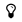
\includegraphics{../manuscript/images/tips}\textbf{TIPS} 

Untuk melakukan casting yang benar, maka casting akan valid jika kita mengcasting tipe data yang berukuran lebih besar menjadi tipe data yang berukuran lebih kecil. Misalnya float dicast menjadi int.
\end{quotation}


\section{Casting Operator pada C++}\label{casting-operator-pada-c}

C++ memiliki cara pengcastingan yang baru, yaitu:

\begin{itemize}

\item
  static\_cast
\item
  dynamic\_cast
\item
  reinterpret\_cast
\item
  const\_cast
\end{itemize}

Bentuk umum untuk semuanya adalah:

\begin{lstlisting}[language=c++, numbers=none]
tipe_tujuan hasil = tipe_casting <tipe_tujuan> (obyek_yg_mau_dicasting);
\end{lstlisting}

\subsection{Pengunaan static\_cast}\label{pengunaan-staticux5fcast}

\emph{Static\_cast} adalah mekanisme yang dapat digunakan untuk
mengkonversi pointer diantara tipe data/class terkait dan melakukan
konversi tipe data tersebut secara eksplisit untuk tipe data standar
yang jika tidak dilakukan konversi akan terjadi secara otomatis
(implisit). Dengan menggunakan konsep pointer, \texttt{static\_cast}
menerapkan pengecekan casting pada saat compile-time dengan melakukan
pemeriksaan untuk memastikan bahwa pointer dicasting ke tipe yang
benar/sesuai. Hal Ini merupakan perbaikan dari casting yang berjenis
C-style, dimana memungkinkan casting ke obyek yang tidak ada relasinya
sama sekali. Dengan menggunakan \texttt{static\_cast}, pointer bisa
dicaskting ke class induknya atau dapat down-case menjadi class
turunannya. Berikut contohnya:

\begin{lstlisting}[language=c++, numbers=none]
CInduk* pInduk = new CTurunan (); // membuat obyek Cturunan dari Cinduk (polymorfisme)
CTurunan* pTurunan = static_cast<CTurunan*>(pInduk); // mengcasting pInduk menjadi Cturunan, valid!
// CTdkAdaHubungan merupakan class yang tidak ada hubungannya dengan CInduk melalui inheritance
CTdkAdaHubungan* pTdkHub = static_cast<CTdkAdaHubungan*>(pInduk); // Error
//karena casting tidak diperbolehkan, tidak ada hubungan class!
\end{lstlisting}

\textbf{Keterangan:}

\begin{itemize}

\item
  Pada contoh diatas terlihat bahwa class anak dapat dibuat dari class
  induk karena ada hubungan pewarisan. Konsep ini merupakan konsep
  polimorfisme. Kemudian untuk memastikan agar tipe data pInduk
  benar/valid untuk dimasukkan ke pTurunan yang merupakan obyek
  CTurunan, maka dilakukan casting dengan static\_casting.
\item
  Kemudian pada bagian kedua, terlihat bahwa jika kita membuat class
  yang tidak ada hubungan apapun dengan class Induk maka kita tidak bisa
  melakukan static\_casting.
\item
  Dengan demikian, static\_casting digunakan untuk meyakinkan validitas
  suatu obyek pointer bahwa obyek tersebut ada hubungan dengan obyek
  yang dicastingnya. Pengcastingan dilakukan dengan mengubah class Induk
  menjadi class Anak, bukan sebaliknya.
\end{itemize}

Bagi para programmer C yang beralih ke C++, static casting sangat mirip
dengan C-style casting dan sangat disarankan untuk mengganti C-style
casting karena static casting lebih aman dan tampak tertulis dengan
jelas. Kita dapat melakukan \texttt{static\_casting} pada tipe data
biasa agar programmer dapat melihat

secara eksplisit tipe data yang dicastingnya. Sintaks umunya adalah:

\begin{lstlisting}[language=c++, numbers=none]
static_cast<<type>>(<value>);
\end{lstlisting}

\textbf{Berikut contohnya:}

\begin{lstlisting}[language=c++, numbers=none]
double myphi = 3.14;
int angka = static_cast<int>(myphi);
\end{lstlisting}

\subsection{Penggunaan dynamic\_cast}\label{penggunaan-dynamicux5fcast}

Fungsi dynamic\_cast merupakan kebalikan dari static\_cast, hal ini
karena proses pengcastingan terjadi saat runtime. Casing jenis ini
sangat tepat untuk digunakan pada class yang memiliki sifat
polimorfisme. Casting ini dapat digunakan untuk melakukan casting secara
aman pada pointer superclass menjadi sebuah pointer subclass dalam
sebuah hierarki kelas. Jika ternyata casting invalid karena tipe obyek
yang dicasting tidak setipe dengan class supernya, maka casting akan
gagal. Agar lebih aman, penggunaan dynamic\_cast sebaiknya digunakan
dalam blok try\ldots{}catch.

\textbf{Bentuk umumnya adalah:}

\begin{lstlisting}[language=c++, numbers=none]
tipe_tujuan* pTujuan = dynamic_cast <tipe_class*> (pSumber);
if (pTujuan) // apakah proses casting sukses?
pTujuan->CallFunc ();
\end{lstlisting}

\textbf{Contoh penggunaan:}

\begin{lstlisting}[language=c++, numbers=none]
CInduk* pInduk = new CTurunan();
// Melakukan down casting
CTurunan* pTurunan = dynamic_cast <CTurunan*> (pInduk);
if (pTurunan) // cek apakah sukses?
pTurunan->CallFungsiClassTurunan ();
\end{lstlisting}

\textbf{Keterangan:}

Pada contoh diatas, kita membuat obyek class Turunan dari class Induk,
kemudian kita melakukan casting ke class Turunan untuk memastikan
validitas obyeknya, kemudian karena sifat pengecekan compiler bersifat
runtime, maka kita bisa memeriksa apakah proses castingnya telah
berjalan dengan sukses atau tidak.

Dynamic\_cast juga dapat digunakan untuk referensi pointer. Caranya
dengan menggunakan tanda \&.

Casting ini tidak boleh menghasilkan kembalian NULL. Sintaksnya:

\begin{lstlisting}[language=c++, numbers=none]
<type> subclass = dynamic_cast<<type> &>( ref_obj );
\end{lstlisting}

\textbf{Contoh:}

\begin{lstlisting}[language=c++, numbers=none]
class CBase { };
class CDerived: public CBase { };
CBase b; CBase* pb;
CDerived d; CDerived* pd;
pb = dynamic_cast<CBase*>(&d); // ok: derived-to-base
pd = dynamic_cast<CDerived*>(&b); // wrong: base-to-derived
\end{lstlisting}

\subsubsection*{Contoh Dynamic Casting.}

Buatlah program berikut:

\begin{lstlisting}[language=c++, caption=Contoh Dynamic Casting]
#include <QtCore/QCoreApplication>
#include <iostream>
using namespace std;
class CAnimal
{
public:
virtual void Bersuara () = 0;
};
class CDog : public CAnimal
{
public:
void KibasEkor () {
cout << "Dog: Kibas-kibas ekor!" << endl;
}
void Bersuara () {
cout << "Dog: Guk-guk!" << endl;
}
};
class CCat : public CAnimal
{
public:
void TangkapTikus () {
cout << "Cat: tikus tertangkap!" << endl;
}
void Bersuara () {
cout << "Cat: Meong!" << endl;
}
};
void TentukanTipeClass (CAnimal* pAnimal);
int main(int argc, char *argv[])
{
QCoreApplication a(argc, argv);
// pAnimal1 berupa obyek Dog
CAnimal* pAnimal1 = new CDog ();
// pAnimal2 berupa obyek Cat
CAnimal* pAnimal2 = new CCat ();
cout << "Penggunaan dynamic_cast untuk menentukan jenis Animal 1" << endl;
TentukanTipeClass(pAnimal1);
cout << "Penggunaan dynamic_cast untuk menentukan jenis Animal 2" << endl;
TentukanTipeClass (pAnimal2);
// Penggunaan virtual function override
cout << "Verifikasi tipe: Animal 1 Besuara!" << endl;
pAnimal1->Bersuara ();
cout << "Verifikasi tipe: Animal 2 Besuara!" << endl;
pAnimal2->Bersuara ();
return a.exec();
}
void TentukanTipeClass (CAnimal* pAnimal)
{
    CDog* pDog = dynamic_cast <CDog*>(pAnimal);
if (pDog)
{
cout << "Binatang Dog!" << endl;
// panggil fungsi dog
pDog->KibasEkor();
}
CCat* pCat = dynamic_cast <CCat*>(pAnimal);
if (pCat)
{
cout << "Binatang kucing!" << endl;
pCat->TangkapTikus();
}
}
\end{lstlisting}

\textbf{Hasil:}

\begin{lcverbatim}
Penggunaan dynamic_cast untuk menentukan jenis Animal 1
Binatang Dog!
Dog: Kibas-kibas ekor!
Penggunaan dynamic_cast untuk menentukan jenis Animal 2
Binatang kucing!
Cat: tikus tertangkap!
Verifikasi tipe: Animal 1 Besuara!
Dog: Guk-guk!
Verifikasi tipe: Animal 2 Besuara!
Cat: Meong!
\end{lcverbatim}
\textbf{Keterangan:}

Kelas abstrak Canimal diturunkan pada dua class, yaitu CDog dan CCat
sehingga memiliki function Berbicara() dimana Dog menggunakannya untuk
menggonggong dan Cat menggunakannya untuk mengeong. Fungsi yang
digunakan adalah dynamic\_cast yang akan menentukan mana method
Berbicara() yang diimplementasikan. Dog akan mengimplementasikan
menggonggong, sedangkan Cat akan mengimplementasikan mengeong. Setelah
mengetahui fungsi mana yang diimplementasikan, method TentukanTipe juga
dapat menggunakan pointernya untuk memanggil method pada class
turunannya sesuai dengan jenis classnya. Untuk class Dog memanggil
method KibasEkor(), sedangkan class Cat memanggil method TangkapTikus().

\subsection{Penggunaan reinterpret\_cast}\label{penggunaan-reinterpretux5fcast}

Penggunaan casting ini benar-benar tidak memungkinkan programmer untuk
mengcasting dari satu obyek ke jenis obyek lain, terlepas dari apakah
jenis obyeknya berhubungan atau tidak. Casting ini tidak boleh digunakan
untuk melakukan down casting pada hierarki kelas atau untuk menghapus
const volatile. Sintaks:

\begin{lstlisting}[language=c++, numbers=none]
reinterpret_cast<<type>>( <val> );
\end{lstlisting}

\textbf{Contoh:}

\begin{lstlisting}[language=c++, numbers=none]
reinterpret_cast<int*>(100);
\end{lstlisting}

Reinterpret\_cast pada class menggunakan syntax sebagai berikut:

\begin{lstlisting}[language=c++, numbers=none]
CInduk * pInduk = new CInduk ();
CTdkAdaHubungan * pTdkHubung = reinterpret_cast<CTdkAdaHubungan*>(pInduk);
// program diatas bisa dikompile tapi sangat tidak disarankan karena class CtdkAdaHubungan bukanlah turunan dari Cinduk.
\end{lstlisting}

Casting model ini sebenarnya memaksa compiler untuk menerima situasi
dimana pada static\_cast tidak diijinkan. Casting model ini biasanya
ditemukan pada pemrograman aplikasi tingkat rendah tertentu (seperti
driver) dimana harus dilakukan konversi ke tipe sederhana dimana API
dapat menerimanya.

\begin{lstlisting}[language=c++, numbers=none]
CSomeClass* pObject = new CSomeClass ();
// harus dikirimkan dalam bentuk byte (unsigned char)
unsigned char* pBytes = reinterpret_cast <unsigned char*>(pObject);
\end{lstlisting}

\textbf{Contoh lain:}

\begin{lstlisting}[language=c++, numbers=none]
class A {};
class B {};
A * a = new A;
B * b = reinterpret_cast<B*>(a);
\end{lstlisting}

\begin{quotation}
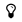
\includegraphics{../manuscript/images/tips.png} \textbf{TIPS} 

Sebisa
mungkin reinterpret\_cast tidak digunakan jika tidak terpaksa karena
tidak aman.
\end{quotation}


\subsection{Penggunaan const\_cast}\label{penggunaan-constux5fcast}

Const\_cast digunakan untuk menghilangkan sifat const-ness atau sifat
volatile-an dari sebuah variabel. Const\_cast harus digunakan dengan
tepat. Salah satu contoh penggunaan yang sah dari const\_cast adalah
untuk menghilangkan sifat const-an dari sebuah pointer agar dapat lulus
menjadi fungsi ketika kita yakin fungsi tersebut tidak akan memodifikasi
variabel tetapi fungsi itu didesain untuk tidak menentukan inputan
sebagai konstanta.

\textbf{Sintaks:}

\begin{lstlisting}[language=c++, numbers=none]
const_cast<<type>>(<value>);
\end{lstlisting}

\textbf{Contoh:}

\begin{lstlisting}[language=c++, numbers=none]
void func(char *);
const char *x = "abcd";
func(const_cast<char *>(x));
\end{lstlisting}

const\_cast juga memungkinkan kita untuk menonaktifkan method const pada
suatu objek. Mengapa diperlukan? Karena kadang-kadang programmer
melupakan penggunaan const pada method yang seharusnya berjenis const
method. Contoh:

\begin{lstlisting}[language=c++, numbers=none]
ContohClass
{
public:
// ...
void tampilkanAnggota (); // method ini berjenis const
};
void tampilkanData (const ContohClass& mData)
{
mData.tampilkanAnggota (); // compile error, karena "call to a non-const member using
a const reference"
}
\end{lstlisting}

Kita dapat menggunakan const\_cast untuk mengubah a adalah:

\begin{lstlisting}[language=c++, numbers=none]
void tampilkanData (const ContohClass& mData)
{
ContohClass& refData = const_cast <ContohClass&>(mData);
refData.tampilkanAnggota(); // OK!
}
\end{lstlisting}

Kita juga dapat menggunakan pointer:

\begin{lstlisting}[language=c++, numbers=none]
void tampilkanData (const ContohClass* pData)
{
// pData->DisplayMembers(); Error: attempt to invoke a non-const function!
CSomeClass* pCastedData = const_cast <CSomeClass*>(pData);
pCastedData->DisplayMembers(); // Allowed!
}
\end{lstlisting}

Contoh lain:

\begin{lstlisting}[language=c++, numbers=none]
// const_cast
#include <iostream>
using namespace std;
void print (char * str)
{
cout << str << endl;
}
int main () {
const char * c = "sample text";
print ( const_cast<char *> (c) );
return 0;
}
\end{lstlisting}

\section{Pemrograman Basisdata dengan QtConsole Application}\label{pemrograman-basisdata-dengan-qtconsole-application}

Pada bagian kedua ini kita akan berkenalan dengan bagaimana mengakses
basisdata dengan menggunakan Qt. Basis data adalah suatu kumpulan
tabel-tabel yang berisi data-data yang saling berelasi satu sama lain
secara logika. Basis data tersusun dari tabel, sedangkan tabel tersusun
dari baris record-record yang memiliki atribut (kolom) dan nilainya.
Gambaran basis data pada Qt Creator seperti gambar \ref{fig:basis-data-qt}

\begin{figure}
\centering
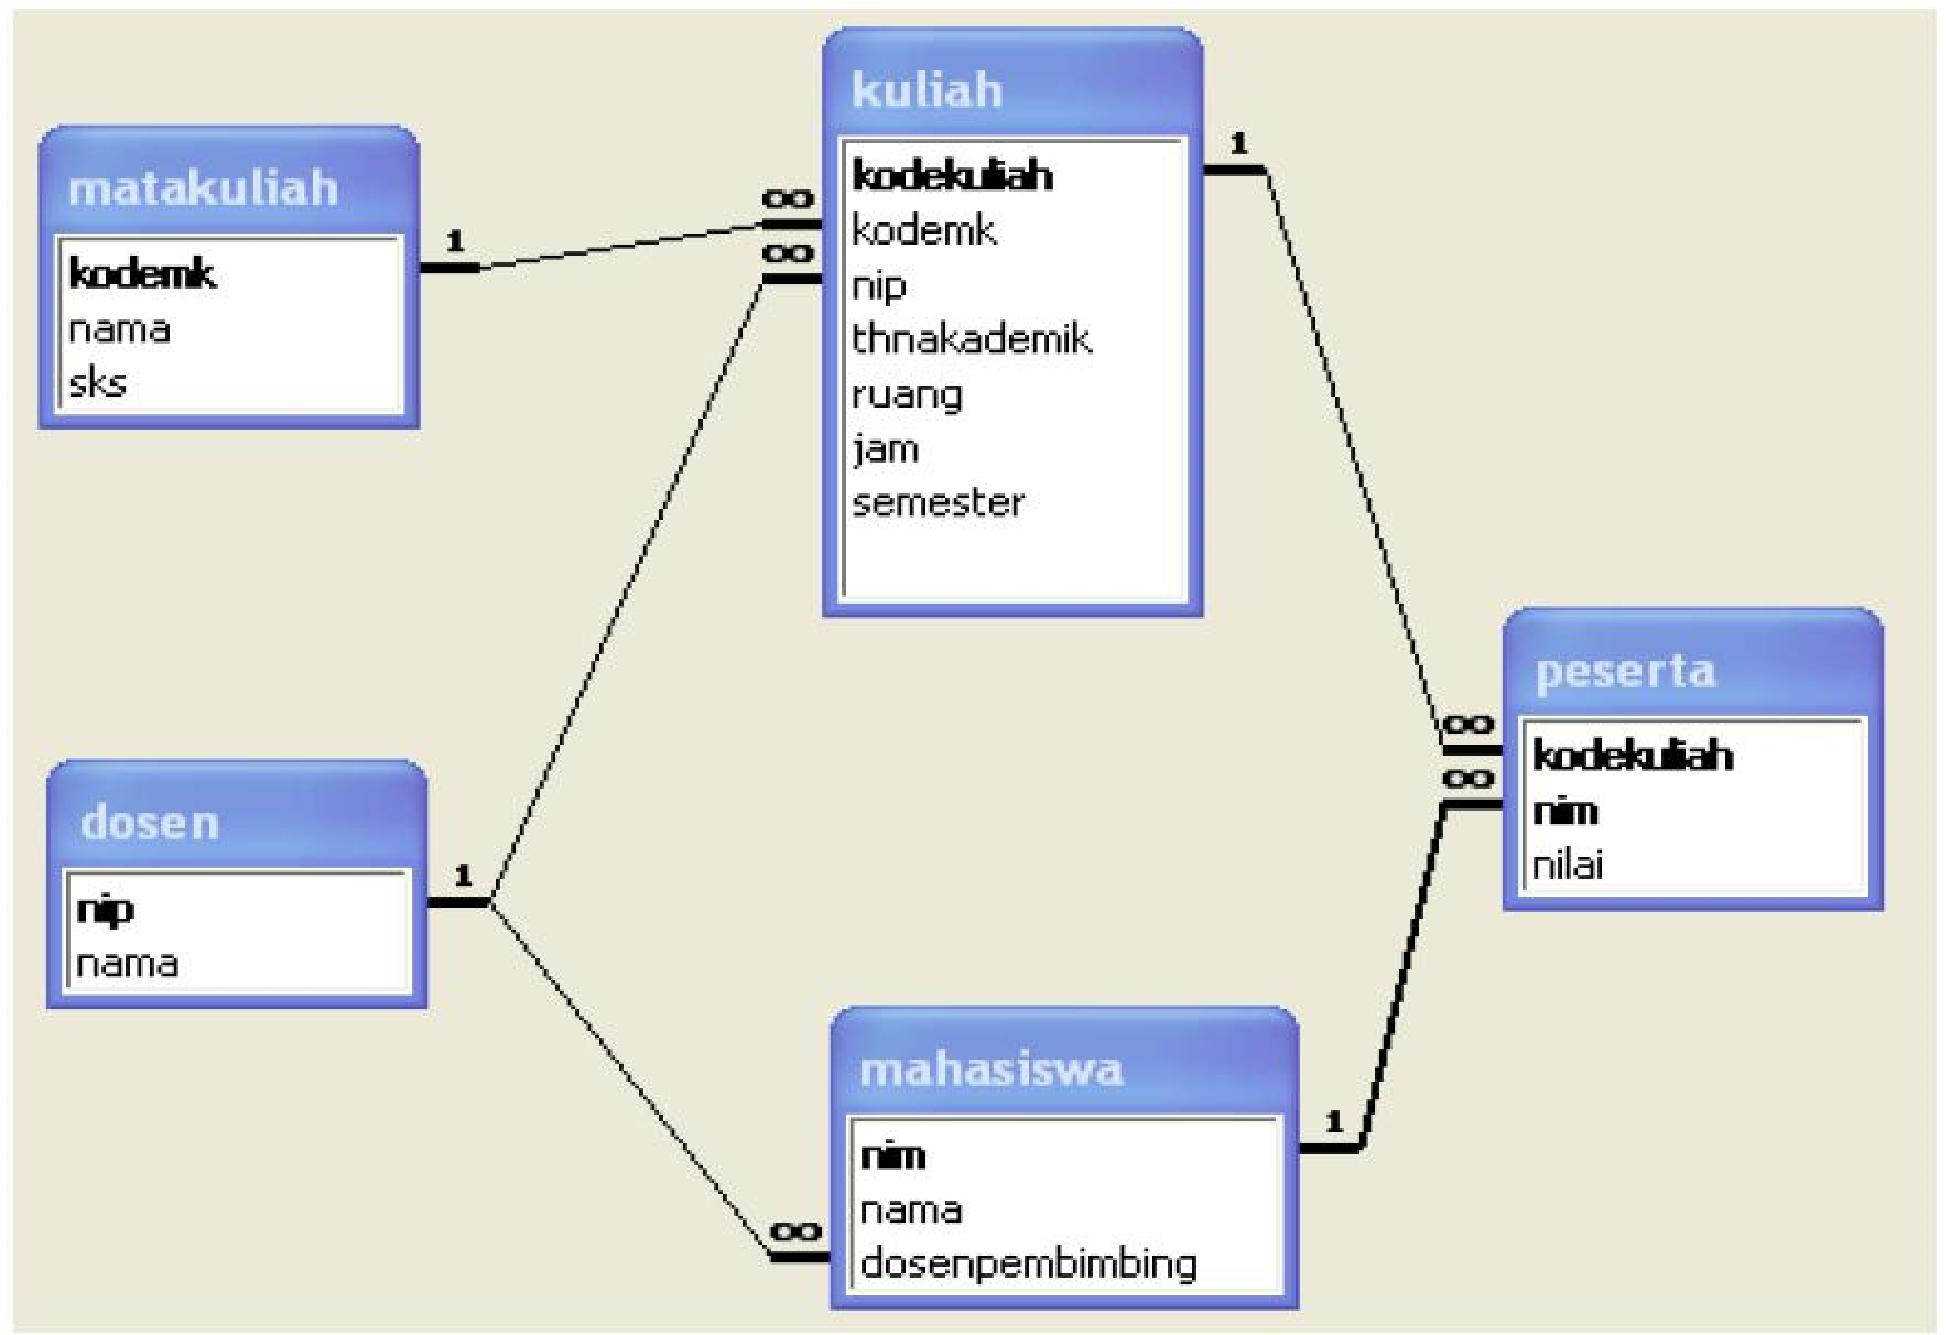
\includegraphics[width=0.7\linewidth]{../manuscript/images/basis-data-qt}
\caption{Pemrograman Basis data Qt Creator}
\label{fig:basis-data-qt}
\end{figure}


Pada contoh diatas, terdapat sebuah basisdata perkuliahan, dimana
terdapat 5 buah tabel. Tabel yang ada memiliki field (atribut/kolom).
Field pada masing-masing tabel sangat berasosiasi dengan tabelnya,
artinya kodemk, nama, dan sks pada tabel matkuliah sangat spesifik
menggambarkan tabel matakuliah, demikian juga yang lainnya.

Kita tidak akan membahas lebih lanjut tentang basisdata. Pada basis data
kita juga mengenal SQL (Structured Query Language). SQL merupakan bahasa
untuk mengakses dan memanipulasi basis data terutama isi record-record
pada tabel.

\subsection{Koneksi Qt dengan Basisdata}\label{koneksi-qt-dengan-basisdata}

Untuk melakukan koneksi pada basis data, Qt menyediakan dukungan pada
beberapa basis data yang terkenal, misalnya
\href{https://www.sqlite.org/about.html}{Sqlite},
\href{https://en.wikipedia.org/wiki/Oracle_Database}{Oracle},
\href{https://www.mysql.com/about/}{MySQL}, Db2\footnote{\href{https://en.wikipedia.org/wiki/IBM_DB2}{IBM
  DB2} adalah produk database server yang dikembangkan oleh IBM.
  Produk-produk ini mendukung sistem manajemen basis data relasional
  (relational DBMS), namun belakangan ini sudah mendukung pula sistem
  manajemen basis data berbasis object-relational (object-relational
  DBMS) dan juga non-relational seperti XML.}, ODBC\footnote{Open
  Database Connectivity (ODBC) adalah Application Programming interface
  (API) database yang khusus digunakan untuk mengakses database
  relasional. ODBC terdapat dalam setiap komputer yang menggunakan
  sistem operasi windows, karena ODBC merupakan bagian dari Windows Open
  System Architecture (WOSA). Dalam ODBC disediakan berbagai Application
  Programming Interface (API) yang berguna untuk menyediaan dan
  memberikan stkitar bagi berbagai kegiatan pemrograman. Keuntungan
  utama menggunakan ODBC ini adalah fleksibilitas, fleksibel disini
  artinya pengubahan jenis database yang dipergunakan oleh sebuah
  aplikasi tidak akan mempengaruhi kode program aplikasi tersebut.}, dan
\href{https://id.wikipedia.org/wiki/PostgreSQL}{Postgresql}. Secara
default basis data yang didukung adalah Sqlite dan ODBC saja, sedangkan
untuk basis data lainnya harus menggunakan driver yang biasanya harus
didownload pada situsnya secara langsung.

Pada Qt kita dapat membuat aplikasi console yang terkoneksi dengan basis
data. Koneksi terhadap kedua database tersebut tidak perlu melakukan
konfigurasi dan mendownload driver tertentu. Pada tulisan ini kita akan
menggunakan basis data Sqlite.

\subsection{Koneksi Qt dengan MySQL dan menampilkan
datanya}\label{koneksi-qt-dengan-mysql-dan-menampilkan-datanya}

\href{https://www.mysql.com/}{MySQL} merupakan database yang sudah
disupport oleh Qt. Untuk membuat database MySQL.

Untuk melakukan koneksi QtConsole dengan MySQL, maka lakukan Contoh
berikut:

\subsubsection*{Contoh Percobaan koneksi MySQL dengan QtConsole}

\begin{enumerate}


\item
  Buatlah sebuah database pada MySQL dengan nama: testmhs
\item
  Gunakan gunakan PHPmyAdmin untuk membuat tabel database.
  
  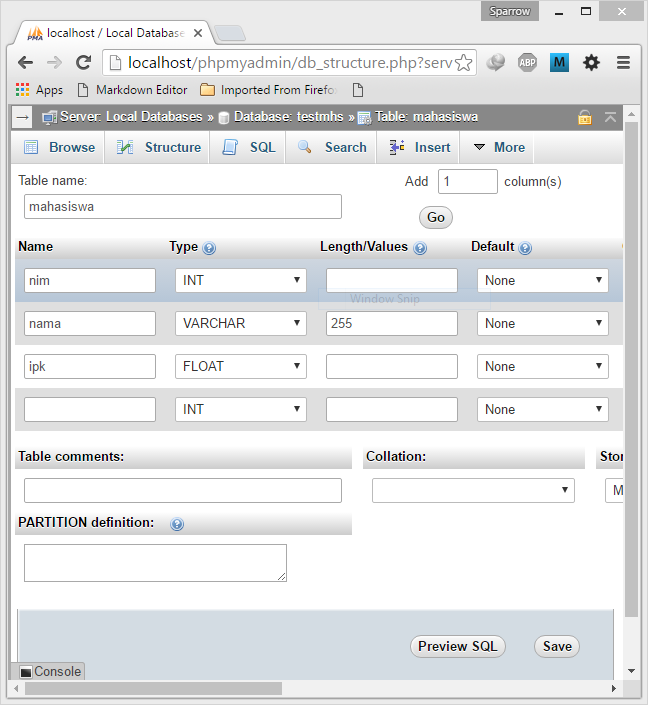
\includegraphics[width=0.7\linewidth]{../manuscript/images/phpmyadmin}
  
\item
  Isilah datanya sebagai berikut:

\begin{longtable}[]{@{}lll@{}}
\toprule
NIM & Nama & IPK\tabularnewline
\midrule
\endhead
011041 & Wachid & 3.6\tabularnewline
012042 & Arif & 3.6\tabularnewline
011012 & Eko & 3.4\tabularnewline
\bottomrule
\end{longtable}

Hasil:

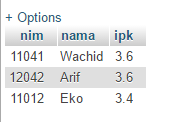
\includegraphics[width=0.7\linewidth]{../manuscript/images/database-mhs}

\item
  Tulis kode berikut ini:


\begin{lstlisting}[language=c++, caption=Percobaan koneksi MySQL dengan QtConsole]
#include <QtCore/QCoreApplication>
#include <QtSql/QtSql>
#include <QtDebug>
int main(int argc, char *argv[])
    {
QCoreApplication a(argc, argv);
qDebug() << QSqlDatabase::drivers();
QSqlDatabase db = QSqlDatabase::addDatabase("QMYSQL");
db.setDatabaseName( "testmhs" );
db.setHostName("localhost");
db.setUserName("root");
db.setPassword("");
if( !db.open() )
{
qDebug() << db.lastError();
qFatal( "Failed to connect." );
} else {
qDebug() << "Koneksi sukses";
QSqlQuery query(db);
query.exec("SELECT * FROM mahasiswa");
while (query.next()) {
qDebug() << query.value(0).toString();
qDebug() << query.value(1).toString();
qDebug() << query.value(2).toString();
}
}
return a.exec();
}
\end{lstlisting}

\item
  Pada file project yang berekstensi .pro, tambahkan linking ke library
  sql sebagai berikut:
  
  \begin{lstlisting}[language=c++]
#-------------------------------------------------
#
# Project created by QtCreator 2016-01-03T19:58:33
#
#-------------------------------------------------
QT += core
QT += gui
Qt += sql
TARGET = databases
CONFIG += console
CONFIG -= app_bundle
TEMPLATE = app
SOURCES += main.cpp
  \end{lstlisting}
\item
  Kemudian run dan hasilnya adalah sebagai berikut:

\begin{lcverbatim}
("QSQLITE", "QMYSQL", "QODBC3", "QODBC")
Koneksi sukses
"11041"
"Wachid"
"3.6"
"12042"
"Arif"
"3.6"
"11012"
"Eko"
"3.4"
\end{lcverbatim}
\end{enumerate}

\textbf{Keterangan:}

\begin{itemize}

\item
  Program diatas dapat menampilkan driver database yang terinstall dan
  dapat dikenali oleh system Qt, yaitu QSQLITE, QMYSQL, QODBC3, dan
  QODBC. Berarti sistem QT dapat mendukung basisdata Sqlite, MySQL, dan
  ODBC dari Microsoft.
\item
  Kemudian langkah pertama yang harus dilakukan adalah membuat
  QsqlDatabase yang akan meload basis data yang dipilih beserta dengan
  drivernya. Setelah itu kita harus menentukan nama database yang akan
  diakses, user, password, dan host lokasi MySQL server.
\item
  Kemudian akan diperiksa apakah database yang terpilih dapat dibuka
  atau tidak dengan method open(). Jika berhasil maka akan dilanjutkan,
  jika tidak maka akan ditampilkan error yang terjadi dengan menggunakan
  method dari database, yaitu lastError().
\item
  Langkah berikutnya adalah melakukan query dengan menggunakan method
  query(). Setelah perintah SQL dijalankan maka record-record yang
  dihasilkan dari perintah select tersebut akan diloop satu persatu
  dengan method next() dari query, dan ditampilkan hasilnya dilayar.
\end{itemize}

\subsection{Koneksi Qt dengan SQLite}\label{koneksi-qt-dengan-sqlite}

SQLite merupakan database yang sudah disupport secara native oleh Qt.
Untuk membuat database SQLite, kita membutuhkan tool yang dapat
digunakan untuk mengelola databasenya dengan mudah, silahkan gunakan
sqliteadmin\footnote{http://www.sqliteexpert.com/} yang berbasis desktop.

Yang perlu diperhatikan ketika kita membuat koneksi dengan basisdata
SQLite adalah:

\begin{enumerate}


\item
  Jika basis data SQLite akan dibuat langsung dari program, maka file
  database hasil pembuatan tersebut akan berada di folder simulator pada
  project kita.
\item
  Jika kita sudah memiliki file database SQLite, maka file tersebut
  harus diletakkan (dikopikan) ke folder simulator atau simulator \textfractionsolidus debug
\item
  File SQLite yang dibuat harus berjenis SQLite 3 agar bisa diakses.
\end{enumerate}

Untuk melakukan koneksi QtConsole dengan SQLite, maka lakukan Contoh
berikut:

\subsubsection*{Contoh Percobaan koneksi SQLite dengan QtConsole}

\begin{enumerate}


\item
  Buatlah sebuah database pada Sqlite dengan nama: testmhs.db, ingat
  harus berjenis SQLite3.

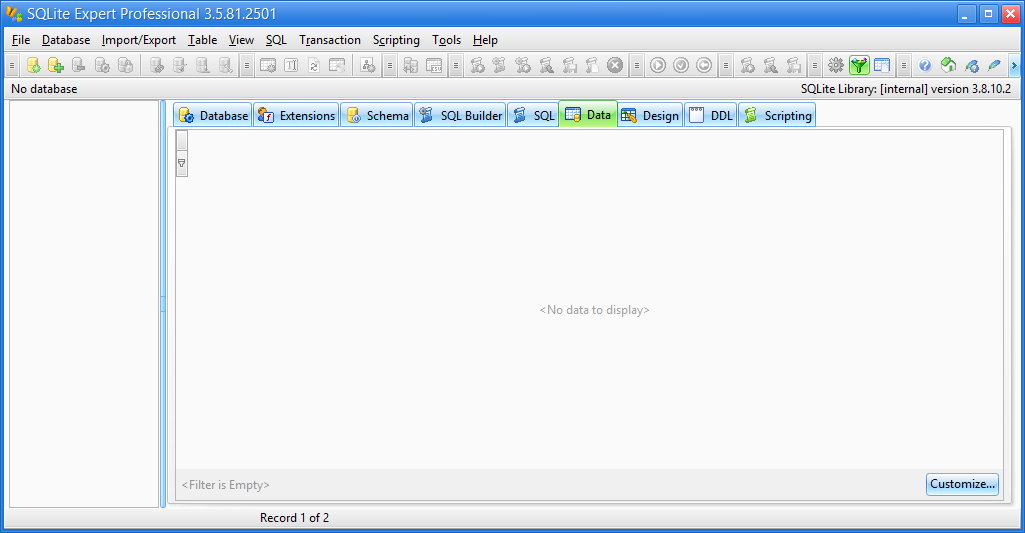
\includegraphics[width=0.7\linewidth]{../manuscript/images/sqlite-expert}
  
  
\item
  Gunakan Sqlite Expert untuk membuatnya
\item
  Pilih menu File \textgreater{} New Database
  
  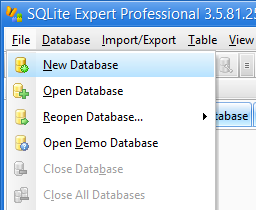
\includegraphics[width=0.7\linewidth]{../manuscript/images/file-new-database}
  
\item
  Simpan dengan nama testmhs.db (pilih tipe sqlite 3 database), simpan
  pada folder project yang akan dibuat.
\item
  Kemudian buat tabel baru dengan klik menu table \textgreater{} New Table,
  kemudian isikan data berikut:

Nama tabel: mahasiswa

Field:

\begin{itemize}

\item
  NIM tipe VARCHAR(8), primary key, not null, unique
\item
  Nama tipe VARCHAR(30), not null
\item
  IPK tipe FLOAT
\end{itemize}


\item
  Kemudian isi data sebagai berikut:


\begin{longtable}[]{@{}lll@{}}
\toprule
NIM & Nama & IPK\tabularnewline
\midrule
\endhead
011041 & Wachid & 3.6\tabularnewline
012042 & Arif & 3.6\tabularnewline
011012 & Eko & 3.4\tabularnewline
\bottomrule
\end{longtable}


\item
  Setelah itu buatlah project baru pada QtConsole application, dan
  tulislah kode program berikut:

\begin{lstlisting}[language=c++, caption=Percobaan koneksi SQLite dengan QtConsole]
#include <QtCore/QCoreApplication>
#include <QDebug>
#include <QtSql/QtSql>
    int main(int argc, char *argv[])
{
QCoreApplication a(argc, argv);
qDebug() << QSqlDatabase::drivers();
QSqlDatabase db = QSqlDatabase::addDatabase("QSQLITE");
db.setDatabaseName( "testmhs.db" );
if( !db.open() )
{
qDebug() << db.lastError();
qFatal( "Failed to connect." );
} else qDebug() << "Koneksi berhasil";
return a.exec();
}
\end{lstlisting}

\item
  Pada project, pilihlah file berekstensi .pro, kemudian bukalah file
  tersebut dan tambahkanlah bagian kode berikut:
  
  \begin{lstlisting}[language=c++]
  #-------------------------------------------------
  #
  # Project created by QtCreator 2016-01-03T19:58:33
  #
  #-------------------------------------------------
  QT += core
  QT += gui
  Qt += sql
  TARGET = databases
  CONFIG += console
  CONFIG -= app_bundle
  TEMPLATE = app
  SOURCES += main.cpp
  \end{lstlisting}
  
\item
  Build dan run

\begin{lcverbatim}
("QSQLITE")
Koneksi berhasil
\end{lcverbatim}
\end{enumerate}

\textbf{Keterangan:}

\begin{itemize}

\item
  Baris pertama output adalah daftar driver yang didukung oleh Qt dan
  QtCreator.
\item
  Baris kedua adalah menggambarkan bahwa koneksi terhadap database
  Sqlite berhasil!
\item
  Program diatas mengharuskan adanya urutan perintah yang harus
  dilakukan ketika kita akan melakukan koneksi ke database Sqlite,
  yaitu: 

\begin{itemize}
\item Load driver SQLITE Tambahkan bagian ini
\item setDatabaseName sesuai dengan nama file Sqlite yang akan diakses 
\item Kemudian open koneksi dengan memanggil method open 
\item Jika ada error tampilkan errornya, jika tidak tampilkan bahwa koneksi berhasil
\end{itemize}  

\end{itemize}

\subsection{Membaca data pada tabel SQLITE}

Cara membaca data pada tabel Sqlite adalah dengan menggunakan perintah
query SQL SELECT. Sintaksnya adalah
\texttt{SELECT\ \textless{}field,\ field,\ field\textgreater{}\ FROM\ \textless{}nama\_tabel\textgreater{}\ WHERE\ \textless{}kondisi\textgreater{}}
Perintah diatas bisa menghasilkan record atau malah salah sekali tidak
menghasilkan record apapun. Jika menghasilkan record, maka record yang
dihasilkan bisa satu atau lebih dari satu.

Pada Qt cara yang digunakan untuk membaca data adalah dengan menggunakan
class QSqlQuery dan method query seperti berikut ini:

\begin{lstlisting}[language=c++, numbers=none]
QSqlQuery query("SELECT * FROM mahasiswa");
while (query.next()) {
QString nim = query.value(0).toString();
qDebug() << nim;
}
\end{lstlisting}

Kita ingat bahwa tabel mahasiswa memiliki 3 kolom: NIM, Nama, dan IPK.

Perintah diatas menggunakan QsqlQuery yang menerima parameter Qstring.
Setelah query dijalankan maka akan dilakukan proses looping untuk
mengambil data-data per baris record dengan menggunakan method next()
dari query. Di dalam looping kita mengambil variabel nim pada kolom
pertama (dalam hal ini digunakan indeks 0). Untuk mengambil field
tertentu pada tabel, misalnya ipk, maka hanya perlu mengganti indeksnya
menjadi 2 saja.

\subsubsection*{Contoh  Membaca data pada Sqlite.}

Tulislah program berikut:

\begin{lstlisting}[language=c++, caption= Membaca data pada Sqlite]
#include <QtCore/QCoreApplication>
#include <QDebug>
#include <QtSql/QtSql>
int main(int argc, char *argv[])
{
QCoreApplication a(argc, argv);
qDebug() << QSqlDatabase::drivers();
QSqlDatabase db = QSqlDatabase::addDatabase("QSQLITE");
db.setDatabaseName("testmhs.db");
if(!db.open())
{
qDebug() << db.lastError();
qFatal( "Failed to connect." );
} else qDebug() << "Koneksi berhasil";
    QSqlQuery query;
bool cek = query.exec("select nim,nama from mahasiswa order by nim desc");
qDebug() << cek;
QString nim,nama;
while(query.next())
{
nim = query.value(0).toString();
nama = query.value(1).toString();
qDebug() << nim << " " << nama;
}
return a.exec();
}
\end{lstlisting}

\textbf{Hasil:}

\begin{lcverbatim}
("QSQLITE")
Koneksi berhasil
true
"11041""Wachid"
"12042""Arif"
"11012""Eko"
\end{lcverbatim}

\textbf{Keterangan:}

\begin{itemize}

\item
  Program diatas melakukan koneksi ke SQLite dan kemudian mengirimkan
  query untuk mengambil data-data dari tabel mahasiswa dengan
  menggunakan query SQL select.
\item
  Untuk mendapatkan hasil dari query kita gunakan perulangan dari
  variabel query dan method next(). Didalam perulangan kita ambil
  masing-masing nilai dari tiap-tiap kolom untuk setiap recordnya dengan
  menggunakan query.value().toString()
\item
  Perintah diatas berarti kita mengambil indeks sesuai dengan kolom yang
  diambil dari SQL, yaitu kolom 0 untuk nim, 1 untuk nama dan
  seterusnya.
\end{itemize}

\subsection{Menambah data pada tabel SQLITE}\label{menambah-data-pada-tabel-sqlite}

Cara menambah data pada tabel Sqlite adalah dengan menggunakan perintah
query SQL INSERT. Sintaksnya adalah
\texttt{INSERT\ INTO\ \textless{}namatabel\textgreater{}\ (\textless{}kolom1\textgreater{},\textless{}kolom2\textgreater{},\ dst)\ VALUES\ (\textless{}nilai1\textgreater{},\ \textless{}nilai2\textgreater{}},
dst) Perintah diatas tidak menghasilkan record sama sekali, namun dapat
menghasilkan berapa jumlah record yang terpengaruh (affected rows) dan
juga mengembalikan nilai bool yang akan bernilai true atau false. Nilai
true jika menambahan data berhasil, nilai false jika penambahan data
gagal.

Pada Qt cara yang digunakan untuk menambah data adalah dengan
menggunakan class QSqlQuery dan method query seperti berikut ini:

\begin{lstlisting}[language=c++, numbers=none]
QSqlQuery query;
bool hasil = query.exec("INSERT INTO mahasiswa (nim, nama,ipk) VALUES
('22113344','anton', 3.4)");
if(hasil) qDebug() << "Berhasil"; else qDebug << "gagal";
\end{lstlisting}

Perintah diatas menggunakan QsqlQuery yang menerima parameter sql dalam
tipe data Qstring. Setelah query dijalankan maka akan diperiksa hasil
dari akibat penambahan datanya. Jika berhasil maka akan mengembalikan
nilai true, sedangkan jika gagal maka akan menghasilkan nilai false.

\subsubsection*{Contoh  Menambahkan data pada SQLite.}

Buatlah program berikut:

\begin{lstlisting}[language=c++, caption= Menambahkan data pada SQLite]
#include <QtCore/QCoreApplication>
#include <QDebug>
#include <QtSql/QtSql>
int main(int argc, char *argv[])
{
QCoreApplication a(argc, argv);
qDebug() << QSqlDatabase::drivers();
QSqlDatabase db = QSqlDatabase::addDatabase("QSQLITE");
db.setDatabaseName("testmhs.db");
if(!db.open())
{
qDebug() << db.lastError();
qFatal( "Failed to connect." );
} else qDebug() << "Koneksi berhasil";
QSqlQuery query;
bool hasil = query.exec("insert into mahasiswa(nim,nama,ipk) values
('22334455','mhs baru',3.12)");
if(hasil) qDebug() << "Berhasil ditambahkan"; else qDebug() << "Gagal
ditambahkan";
return a.exec();
}
\end{lstlisting}

\textbf{Hasil:}

\begin{lcverbatim}
("QSLITE")
Koneksi berhasil
Berhasil ditambahkan
\end{lcverbatim}

\textbf{Keterangan:}

\begin{itemize}
\item
  Pada awalnya data pada tabel mahasiswa hanya berjumlah 3 buah data,
  ketika program dijalankan maka data baru bernama ``mhs baru'' berhasil
  ditambahkan dan mengubah jumlah record pada tabel sehingga menjadi 4
  buah. Tampilan perubahan adalah sebagai berikut:
  
  \begin{tabular}{|l|l|l|}
  \hline
  NIM & Nama & IPK \\ \hline
  011041 & Wachid & 3.1 \\ \hline
  012042 & Arif & 3.6 \\ \hline
  011041 & Eko & 3.4 \\ \hline
  012011 & Alif & 3.3 \\ \hline
  013021 & Ananda & 3.8 \\ \hline
  
  \end{tabular}
\item
  Cara menambahkan record pada SQLite sangat mudah, yaitu dengan
  menggunakan SQL insert into yang harus disesuaikan dengan jumlah field
  yang ada pada tabel. Setelah itu query akan dijalankan dengan method
  exec dari obyek QsqlQuery.
\item
  Hasil kembalian dari method exec ini adalah bool yang menghasilkan
  nilai true atau false. Jika menghasilkan nilai true maka record
  berhasil ditambahkan, jika false maka record tidak berhasil
  ditambahkan!
\item
  Jika program diatas dieksekusi sekali lagi (diulangi) maka akan
  menampilkan tulisan Gagal ditambahkan. Hal ini dikarenakan kita
  menambahkan record yang sama persis dengan ebelumnya padahal kita
  sudah menset bahwa field nim bersifat primary, yang artinya tidak
  boleh ada data nim yang kembar. Hal inilah yang menyebabkan data Gagal
  ditambahkan.
  \begin{lcverbatim}
  ("QSLITE")
  Koneksi berhasil
  gagal  ditambahkan
\end{lcverbatim}

\item Jika kita hendak membaca data pada SQLite, maka tambahkan kode berikut:

\begin{lstlisting}[language=c++, caption=Membaca data pada SQLite]
QsqlQuery query.exec("select nim,nama,ipk from mahasiswa order by nim desc");
QString nim,nama;
float ipk;
while(query.next())
{
nim = query.value(0).toString();
nama = query.value(1).toString();
ipk = query.value(2).toFloat();
qDebug() << nim << " " << nama << " " << ipk;
}
\end{lstlisting}

\item Sehingga akan dihasilkan:

\begin{lcverbatim}
"012011"  "Alif"  "3.3"
"013021"  "Ananda"  "3.8" 
"011041" "Wachid"  "3.1" 
"012042"  "Arif"  "3.6" 
"011012"  "Eko"  "3.4" 

\end{lcverbatim}
\end{itemize}



\subsection{Mengedit data pada tabel SQLITE}\label{mengedit-data-pada-tabel-sqlite}

Cara mengedit data pada tabel Sqlite adalah dengan menggunakan perintah
query SQL UPDATE. Sintaksnya adalah
\texttt{UPDATE\ \textless{}namatabel\textgreater{}\ SET\ \textless{}kolom1\textgreater{}=\textless{}nilaikolom1\textgreater{},\textless{}kolom2\textgreater{}=\textless{}nilaikolom2\textgreater{}},
dst \texttt{WHERE\ \textless{}kriteri} Perintah diatas tidak
menghasilkan record sama sekali, namun dapat menghasilkan berapa jumlah
record yang terpengaruh (affected rows) dan juga mengembalikan nilai
bool yang akan bernilai true atau false. Nilai true jika pengeditan data
berhasil, nilai false jika pengeditan data gagal.

Pada Qt cara yang digunakan untuk mengedit data adalah dengan
menggunakan class QSqlQuery dan method query seperti berikut ini:

\begin{lstlisting}[language=c++, caption=menggunakan class QSqlQuery dan method query]
QSqlQuery query;
bool hasil = query.exec("UPDATE mahasiswa SET nama='Antonius Rachmat C' WHERE
nim='2200259');
if(hasil) qDebug() << "Berhasil"; else qDebug << "gagal";
\end{lstlisting}

Perintah diatas menggunakan QsqlQuery yang menerima parameter sql dalam
tipe data Qstring. Setelah query dijalankan maka akan diperiksa hasil
dari akibat pengeditan datanya. Jika berhasil maka akan mengembalikan
nilai true, sedangkan jika gagal maka akan menghasilkan nilai false.

\subsubsection*{Contoh Mengedit data pada SQLite.}

\begin{enumerate}
\item Kondisi awal tabel:

\begin{tabular}{|l|l|l|}
\hline
NIM & Nama & IPK \\ \hline
011041 & Wachid & 3.1 \\ \hline
012042 & Arif & 3.6 \\ \hline
011041 & Eko & 3.4 \\ \hline
012011 & Alif & 3.3 \\ \hline
013021 & \colorbox{red}{Ananda} & 3.8 \\ \hline
\end{tabular}

Kita akan mengedit nim 013021 menjadi bernama Aryo

\item Buatlah program berikut:

\begin{lstlisting}[language=c++, caption=Mengedit data pada SQLite]
#include <QtCore/QCoreApplication>
#include <QDebug>
#include <QtSql/QtSql>
#include <iostream>
using namespace std;
int main(int argc, char *argv[])
{
QCoreApplication a(argc, argv);
qDebug() << QSqlDatabase::drivers();
QSqlDatabase db = QSqlDatabase::addDatabase("QSQLITE");
db.setDatabaseName("testmhs.db");
if(!db.open())
{
qDebug() << db.lastError();
qFatal( "Failed to connect." );
} else qDebug() << "Koneksi berhasil";
QSqlQuery query;
bool hasil = query.exec("update mahasiswa set nama='Antonius Rachmat C' where
nim='22002529'");
if(hasil) qDebug() << "Berhasil diedit"; else qDebug() << "Gagal diedit";
qDebug() << "Jumlah record yang diedit: " << query.numRowsAffected();
return a.exec();
}
\end{lstlisting}

\item \textbf{Hasil:}
\begin{lcverbatim}
("QSLITE")
Koneksi berhasil
Berhasil diedit
Jumlah record yang diedit : 1
\end{lcverbatim}
\item Kondisi akhir tabel:

\begin{tabular}{|l|l|l|}
\hline
013021 & Ananda & 3.8 \\ \hline
NIM & Nama & IPK \\ \hline
011041 & Wachid & 3.1 \\ \hline
012042 & Arif & 3.6 \\ \hline
011041 & Eko & 3.4 \\ \hline
012011 & Alif & 3.3 \\ \hline

\end{tabular}
\end{enumerate}

\textbf{Keterangan:}

\begin{itemize}

\item
  Program diatas masih sama menggunakan obyek QsqlQuery dan method
  exec(). Hanya SQL query nya saja yang berbeda dengan Contoh sebelumnya
  saat penambahan data. SQL query pada saat pengeditan menggunakan SQL
  UPDATE SET.
\item
  Untuk mengetahui berapa jumlah record yang terupdate digunakan method
  numRowsAffected() dari obyek QsqlQuery.
\end{itemize}

\subsection{Menghapus data pada tabel SQLITE}\label{menghapus-data-pada-tabel-sqlite}

Cara menghapus data pada tabel Sqlite adalah dengan menggunakan perintah
query SQL UPDATE. Sintaksnya adalah DELETE FROM WHERE \textless{}kriteri
Perintah diatas tidak menghasilkan record sama sekali, namun dapat
menghasilkan berapa jumlah record yang terpengaruh (affected rows) dan
juga mengembalikan nilai bool yang akan bernilai true atau false. Nilai
true jika penghapusan data berhasil, nilai false jika penghapusan data
gagal.

Pada Qt cara yang digunakan untuk menghapus data adalah dengan
menggunakan class QSqlQuery dan method query seperti berikut ini:

\begin{lstlisting}[language=c++, caption=menghapus data adalah dengan menggunakan class QSqlQuery dan method query]
QSqlQuery query;
bool hasil = query.exec("DELETE FROM mahasiswa WHERE nim='22334455');
if(hasil) qDebug() << "Berhasil"; else qDebug << "gagal";
\end{lstlisting}

Perintah diatas menggunakan QsqlQuery yang menerima parameter sql dalam
tipe data Qstring. Setelah query dijalankan maka akan diperiksa hasil
dari akibat penghapusan datanya. Jika berhasil maka akan mengembalikan
nilai true, sedangkan jika gagal maka akan menghasilkan nilai false.

\subsubsection*{Contoh  Menghapus data pada SQLite.}

\begin{enumerate}
\item Kondisi awal tabel:

\begin{tabular}{|l|l|l|}
\hline
NIM & Nama & IPK \\ \hline
011041 & Wachid & 3.1 \\ \hline
012042 & Arif & 3.6 \\ \hline
011041 & Eko & 3.4 \\ \hline
012011 & Alif & 3.3 \\ \hline
013021 & \colorbox{red}{Ananda} & 3.8 \\ \hline
\end{tabular}

Kita akan menghapus data ``Ananda''.

\item Buatlah program sebagai berikut:

\begin{lstlisting}[language=c++, caption= Menghapus data pada SQLite]
#include <QtCore/QCoreApplication>
#include <QDebug>
#include <QtSql/QtSql>
#include <iostream>
using namespace std;
int main(int argc, char *argv[])
{
QCoreApplication a(argc, argv);
qDebug() << QSqlDatabase::drivers();
QSqlDatabase db = QSqlDatabase::addDatabase("QSQLITE");
db.setDatabaseName("testmhs.db");
if(!db.open())
{
qDebug() << db.lastError();
qFatal( "Failed to connect." );
} else qDebug() << "Koneksi berhasil";
QSqlQuery query;
bool hasil = query.exec("delete from mahasiswa where nim='22334455'");
if(hasil) qDebug() << "Berhasil dihapus"; else qDebug() << "Gagal dihapus";
qDebug() << "Jumlah record yang dihapus: " << query.numRowsAffected();
return a.exec();
}
\end{lstlisting}

\item \textbf{Hasil:}

\begin{lcverbatim}
("QSLITE")
Koneksi berhasil
Berhasil diedit
Jumlah record yang dihapus : 1
\end{lcverbatim}

\item Kondisi akhir tabel:

\begin{tabular}{|l|l|l|}
\hline
NIM & Nama & IPK \\ \hline
011041 & Wachid & 3.1 \\ \hline
012042 & Arif & 3.6 \\ \hline
011041 & Eko & 3.4 \\ \hline
012011 & Alif & 3.3 \\ \hline

\end{tabular}

\end{enumerate}

\textbf{Keterangan:}

Program diatas mampu menghapus data pada suatu record tertentu dengan
menggunakan perintah SQL DELETE FROM. Program diatas tidak ada perubahan
dari Contoh sebelumnya kecuali bagian perintah SQL nya.

Demikianlah kita sudah berlatih sejumlah manipulasi data pada tabel
SQLite dengan menggunakan QtSql. Pada databse lain misalnya MySQL semua
perintah --perintah yang sudah dipelajari dapat digunakan dan hanya
perlu disesuaikan pada bagian koneksi pada databasenya. Pemrograman
basis data pada Qt termasuk mudah.

Pada bagian berikutnya kita akan mencoba membuat program untuk
memanipulasi data pada tabel mahasiswa dengan menggunakan menu. Pada
menu akan ditampilkan beberapa pilihan seperti:

\begin{enumerate}


\item
  Tambah data
\item
  Tampil data
\item
  Hapus data
\item
  Cari nim
\item
  Edit data
\item
  Exit
\end{enumerate}

Penjelasan:

\begin{itemize}

\item
  Menu 1 akan digunakan untuk menambah data mahasiswa
\item
  Menu 2 akan digunakan untuk menampilkan data semua mahasiswa
\item
  Menu 3 akan digunakan untuk menghapus data seorang mahasiswa
  berdasarkan nimnya
\item
  Menu 4 akan digunakan untuk mencari data seorang mahasiswa berdasarkan
  nimnya
\item
  Menu 5 akan digunakan untuk mengedit data seorang mahasiswa
  berdasarkan nimnya
\end{itemize}

Cara yang digunakan adalah dengan membuat sebuah class yang akan
digunakan untuk mengakses semua fungsi yang berhubungan dengan
manipulasi data pada basis data SQLite. Method pada class adalah connect
untuk koneksi database, sebuah konstruktor dan method untuk mengambil
nama tabel serta nama database SQLitenya. Kemudian akan dibuat
fungsi-fungsi lain diluar class yang digunakan untuk melakukan
fungsi-fungsi sesuai dengan 5 fungsi yang didefinisikan pada menu. Untuk
lebih jelasnya silahkan dicoba pada Contoh berikut ini.

\subsubsection*{Contoh  Pembuatan manipulasi data pada SQLite dengan menggunakan menu}

\begin{enumerate}

\item
  Tulislah program berikut:

\begin{lstlisting}[language=c++, caption= Pembuatan manipulasi data pada SQLite dengan menggunakan menu]
#include <QtCore/QCoreApplication>
#include <QDebug>
#include <QtSql/QtSql>
#include <iostream>
#include <conio.h>
using namespace std;
class Tabel{
private:
QString namadb;
QString namatabel;
QString strquery;
QSqlDatabase db;
public:
//konstruktor
Tabel(QString namadb, QString namatabel){
this->namadb = namadb;
this->namatabel = namatabel;
}
bool connect(){
this->db = QSqlDatabase::addDatabase("QSQLITE");
this->db.setDatabaseName(this->namadb);
if(!this->db.open())
{
qDebug() << "No";
return false;
} else {
qDebug() << "Yes";
return true;
}
}
bool jalanQuery(QString query){
this->strquery = query;
bool hasil = false;
if(this->db.isOpen()){
QSqlQuery myq(this->db);
hasil = myq.exec(this->strquery);
}
return hasil;
}
void ambilData(QString query){
this->strquery = query;
if(this->db.isOpen()){
QSqlQuery myq(this->db);
myq.exec(this->strquery);
QSqlRecord rec = myq.record();
int cols = rec.count();
QString temp;
for( int c=0; c<cols; c++ )
temp += rec.fieldName(c) + ((c<cols-1)?"\t":"");
qDebug() << temp;
while( myq.next() )
{
temp = "";
for( int c=0; c<cols; c++ )
temp += myq.value(c).toString() + ((c<cols-1)?"\t":"");
qDebug() << temp;
}
    }
}
QString getNamaTabel(){
return this->namatabel;
}
QString getNamaDb(){
return this->namadb;
}
QSqlDatabase getDb(){
return this->db;
}
};
void tambahData(Tabel t){
string nim,nama,ipk;
getline(cin,nim);
cout << "NIM: "; getline(cin,nim);
cout << "Nama: "; getline(cin,nama);
cout << "IPK: "; getline(cin,ipk);
QString s = "insert into "+t.getNamaTabel()+" values
('"+nim.c_str()+"','"+nama.c_str()+"',"+ipk.c_str()+")";
bool hasil = t.jalanQuery(s);
if(hasil) qDebug() << "Penambahan berhasil"; else qDebug() << "Penambahan gagal";
}
void hapusData(Tabel t){
string nim;
getline(cin,nim);
cout << "NIM yang akan dihapus: "; getline(cin,nim);
QString s = "delete from "+t.getNamaTabel()+" where nim='"+nim.c_str()+"'";
bool hasil = t.jalanQuery(s);
if(hasil) qDebug() << "Penghapusan berhasil"; else qDebug() << "Penghapusan
gagal";
}
void tampilData(Tabel t){
QString s = "select * from "+t.getNamaTabel()+" order by nim asc";
t.ambilData(s);
}
void cariNim(Tabel t){
string nim;
getline(cin,nim);
cout << "NIM yang akan dicari: "; getline(cin,nim);
QString s = "select * from "+t.getNamaTabel()+" where nim='"+nim.c_str()+"'";
t.ambilData(s);
}
void editData(Tabel t){
string nim,nama,ipk;
getline(cin,nim);
cout << "NIM yang akan diedit: "; getline(cin,nim);
cout << "Nama baru: "; getline(cin,nama);
cout << "IPK baru: "; getline(cin,ipk);
QString s = "update "+t.getNamaTabel()+" set
nama='"+nama.c_str()+"',ipk="+ipk.c_str()+" where nim='"+nim.c_str()+"'";
bool hasil = t.jalanQuery(s);
if(hasil) qDebug() << "Pengeditan berhasil"; else qDebug() << "Pengeditan gagal";
}
    int main(int argc, char *argv[])
{
QCoreApplication a(argc, argv);
int pil;
Tabel t("testmhs.db","mahasiswa");
t.connect();
do {
system("cls");
cout << "MENU" <<endl;
cout << "1. Tambah data\n";
cout << "2. Tampil data\n";
cout << "3. Hapus data\n";
cout << "4. Cari nim\n";
cout << "5. Edit data\n";
cout << "6. Exit\n";
cout << "Pilihan : "; cin >> pil;
cout << endl;
switch (pil) {
case 1:
tambahData(t);break;
case 2:
tampilData(t);break;
case 3:
hapusData(t);break;
case 4:
cariNim(t);break;
case 5:
editData(t);
}
cout << "Tekan sembarang tombol..."; getch();
} while (pil >=1 && pil<=5);
cout << "Good bye";
return a.exec();
}
\end{lstlisting}
\end{enumerate}

\textbf{Hasil:}

\begin{enumerate}

\item
  Tampilan menu:
  
 \begin{lcverbatim}
MENU:
1. Tambah data
2. Tampil data
3. Hapus data
4. Cari nim
5. Edit data
6. Exit
Pilihan:
 \end{lcverbatim}

\item
  Menu tambah data dan tampil data:
  
 \begin{lcverbatim}
 MENU:
 1. Tambah data
 2. Tampil data
 3. Hapus data
 4. Cari nim
 5. Edit data
 6. Exit
 Pilihan: 1
 NIM: 013012
 Nama: Ramadhani
 Penambahan berhasil
 Tekan sembarang tombol . . .
 \end{lcverbatim}
  
\begin{lcverbatim}
"NIM  Nama  IPK" 
"011041  Wachid  3.1" 
"012042  Arif  3.6 "
"011041  Eko  3.4"
"012011  Alif  3.3" 
"013012 Ramadhani   3.8" 
  \end{lcverbatim}
\item
  Menu hapus data dan tampil data:
  
 \begin{lcverbatim}
MENU:
1. Tambah data
2. Tampil data
3. Hapus data
4. Cari nim
5. Edit data
6. Exit
Pilihan: 3
NIM yang akan dihapus: 011041
Penghapusan berhasil
Tekan sembarang tombol . . .
\end{lcverbatim}
\begin{lcverbatim}
"NIM  Nama  IPK" 
"012042  Arif  3.6 "
"011041  Eko  3.4"
"012011  Alif  3.3" 
"013012 Ramadhani   3.8" 
\end{lcverbatim}
   
\item
  Menu edit data dan tampil data: 
  
  Mengedit 011041 menjadi bernama
  Nur Wachid dan IPK menjadi 3.01
  
  \begin{lcverbatim}
  MENU:
  1. Tambah data
  2. Tampil data
  3. Hapus data
  4. Cari nim
  5. Edit data
  6. Exit
  Pilihan: 5
  NIM yang akan diedit: 011042
  Nama baru: Arif H
  IPK: 3.01
  Tekan sembarang tombol . . .
  \end{lcverbatim}
  
\begin{lcverbatim}
"NIM  Nama  IPK" 
"012042  Arif H  3.6 "
"011041  Eko  3.4"
"012011  Alif  3.3" 
"013012 Ramadhani   3.8" 
\end{lcverbatim}
\item
  Menu cari data:

\begin{lcverbatim}
MENU:
1. Tambah data
2. Tampil data
3. Hapus data
4. Cari nim
5. Edit data
6. Exit
Pilihan: 4
NIM yang akan dicari: 011042
"NIM  Nama  IPK" 
"012042  Arif H  3.6 "
Tekan sembarang tombol . . .
\end{lcverbatim}
\item
  Menu Exit

\begin{lcverbatim}
MENU:
1. Tambah data
2. Tampil data
3. Hapus data
4. Cari nim
5. Edit data
6. Exit
Pilihan: 6
Tekan sembarang tombol . . .Good bye
\end{lcverbatim}

\end{enumerate}

\textbf{Keterangan:}

\begin{itemize}

\item
  Program diatas merupakan program yang cukup banyak dan kompleks.
  Program ini dibuat dengan prinsip perulangan. Kita akan mengulang
  terus menerus bagian menu 1-6 sampai pengguna menginputkan angka yang
  bukan diantara 1-5. Jika pengguna memasukkan angka 1 maka dipanggil
  menu pertama, dan seterusnya. Jika pengguna memasukkan angka 6 maka
  program akan menampilkan Good Bye.
\item
  Pada awal program kita membuat sebuah class bernama Tabel yang
  digunakan untuk mengelola data-data pada tabel mahasiswa. Class Tabel
  harus diinisialisasi terlebih dahulu pada method int main() dengan
  mengiputkan nama database dan nama tabelnya. Setelah diinisialisai
  maka class Tabel harus melakukan method connect agar database SQLite
  terbuka (open).
\item
  Ketika menu penambahan data dipilih, maka method tambahData akan
  dipanggil dan membutuhkan parameter Tabel yang sudah dibuat dan
  diinisialisasi terlebih dahulu sebelumnya. Setelah itu berdasarkan
  obyek Tabel yang sudah dibuat, kita akan menggunakannya untuk
  memasukkan data.
\item
  Pada menu tambah, program akan meminta inputan nim, nama, dan ipk
  kepada pengguna. Setelah pengguna mengiputkan data dengan lengkap,
  maka method tambahData() akan dipanggil sehingga data dapat masuk ke
  tabel. Proses memasukkan data dilakukan dengan menggunakan query
  INSERT.
\item
  Demikian pula dengan menu tampil data, method yang digunakan sama pada
  contoh-contoh sebelumnya, namun ditambah dengan cara membaca
  kolom-kolom pada tabel dan menampilkan semua recordnya satu persatu
  dengan perulangan.
\item
  Pada menu hapus data, perintah yang digunakan juga hanya mengubah
  query SQLnya.
\item
  Pada menu cari data, kita juga menggunakan SQL select seperti pada
  menampilkan data. Perbedaannya hanyalah kondisi where yang digunakan.
  Pada menu pencarian data, kita mencari satu buah record mahasiswa saja
  berdasarkan nimnya.
\item
  Pada menu edit data, kita juga menggunakan SQL update yang dapat
  digunakan untuk mengubah data pada tabel. Pada menu edit ini, kita
  mencari terlebih dahulu nim mahasiswa yang akan diedit baru
  mengeditnya.
\end{itemize}

\begin{quotation}

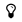
\includegraphics{../manuscript/images/tips}\textbf{TIPS:} 

Untuk
mengkonversi dari tipe data string menuju ke Qstring, digunakan
\texttt{\textless{}variabel\ string\ bias.c\_str()} Perintah cin tidak
bisa digunakan setelah fungsi getline, karena akan membuat inputan
menjadi bertumpuk seperti pada contoh ini:

\begin{lstlisting}[language=c++, numbers=none]
int main(){
int id, age;
string name, address;
cout<<"Enter ID : "; cin>>id;
cout<<"Enter Name: "; getline(cin,name);
cout<<"Enter Address : "; getline(cin, address);
cout<<"Enter Age: "; cin>>age;
}
\end{lstlisting}

\textbf{Hasil:}

\begin{lcverbatim}
Enter ID: 23
Enter Name: Enter Address : Yogyakarta
Enter Age : 45
\end{lcverbatim}

Terlihat bahwa Enter Name dan Enter Address tergabung dan menjadi satu.
Untuk mencegahnya kita bisa menukar posisi bahwa cin diletakkan dibawah
getline, seperti berikut:

\begin{lstlisting}[language=c++, numbers=none]
int main(){
 int id, age;
 string name, address;
 cout<<"Enter Name: "; getline(cin,name);
 cout<<"Enter Address : "; getline(cin, address);
 cout<<"Enter ID : "; cin>>id;
 cout<<"Enter Age: "; cin>>age;
 }
\end{lstlisting}

\textbf{Sehingga tampilan:}

\begin{lcverbatim}
Enter Name: Yanuar Adi
Enter Address : Yogyakarta
Enter ID: 23
Enter Age: 43
\end{lcverbatim}

Jika cin tetap harus didahulukan sebelum getline, maka bisa dilakukan
dengan cara:

\begin{lstlisting}[language=c++, numbers=none]
int main(){
int id, age;
string name, address;
cout<<"Enter ID : "; cin>>id;
getline(cin,name);
cout<<"Enter Name: "; getline(cin,name);
cout<<"Enter Address : "; getline(cin, address);
cout<<"Enter Age: "; cin>>age;
}
\end{lstlisting}

\textbf{Sehingga tampilan:}

\begin{lcverbatim}
Enter ID : 23
Enter Name : Yanuar Adi
Enter Address : Yogyakarta
Enter Age : 32
Terimakasih.
\end{lcverbatim}
\end{quotation}

